\documentclass{article}
\usepackage[T1]{fontenc}

\usepackage{float}
\usepackage{aliascnt}
\newaliascnt{eqfloat}{equation}
\newfloat{eqfloat}{h}{eqflts}
\floatname{eqfloat}{Equation}

\newcommand*{\ORGeqfloat}{}
\let\ORGeqfloat\eqfloat
\def\eqfloat{%
  \let\ORIGINALcaption\caption
  \def\caption{%
    \addtocounter{equation}{-1}%
    \ORIGINALcaption
  }%
  \ORGeqfloat
}
\usepackage{siunitx} % Provides the \SI{}{} and \si{} command for typesetting SI units
\usepackage{graphicx} % Required for the inclusion of images
\usepackage{natbib} % Required to change bibliography style to APA
\usepackage{amsmath} % Required for some math elements 
\usepackage[portuges]{babel}
\usepackage[utf8]{inputenc}
\usepackage{longtable}
\usepackage[table,xcdraw]{xcolor}
\usepackage{caption}
\usepackage{subcaption}
\setlength\parindent{0pt} % Removes all indentation from paragraphs

\renewcommand{\labelenumi}{\alph{enumi}.} % Make numbering in the enumerate environment by letter rather than number (e.g. section 6)

%\usepackage{times} % Uncomment to use the Times New Roman font

%----------------------------------------------------------------------------------------
%	DOCUMENT INFORMATION
%----------------------------------------------------------------------------------------

\title{Princípio do Mínimo da Energia Potencial Total aplicado a deformação de uma estrutura treliçada do tipo cantilever	} % Title

\author{Luis Vinicius Costa Silva}
\date{\today}
\begin{document}
\maketitle
\nocite{*} 
\begin{center}
\begin{tabular}{l r}
Disciplina: & Otimização Clássica \\
Professor: & Romes Antônio Borges
\end{tabular}
\end{center}

\section{Introdução}
Este trabalho tem como objetivo criar um modelo matemático que permita representar a deformação de uma estrutura dada sua configuração inicial. Foi utilizada uma abordagem da otimização clássica que se baseia no Princípio do mínimo da Energia Potencial. \newline
Para tanto, fez-se a modelagem de uma viga treliçada do tipo cantilever, e a obtenção das equações constitutivas do sistema e a escrita do problema em forma de problema de otimização. Posteriormente foi escrito um código computacional (em linguagem Python) para a resolução computacional do problema, isto é: dada uma configuração inicial da estrutura, minimizar a Função de Energia Potencial Total do sistema, obtendo os valores das variáveis de estados (configuração final da estrutura) associada a energia potencial mínima do sistema.\newline
Foram utilizados três algoritmos clássicos para a resolução do problema de otimização: L-BFGS-B, SLSQP e Newton Truncado. Além disso foi utilizado a Evolução Diferecial como algoritmo evolutivo para a resolução do problema. Os resultados obtidos por tais algoritmos foram comparados em um estudo de caso, avaliando as vantagens e desvantagens de cada um deles para o problema em questão.
\section{Modelagem}
\subsection{Princípio do mínimo da Energia Potencial \\ Total}
O Princípio do mínimo da Energia Potencial dita que o estado de equilíbrio mecânico de um sistema é aquele que (de todas as alternativas possíveis) tem a menor energia potencial (basicamente uma reformulação da segunda lei da Termodinâmica) (\cite{reddy2007introduction}). A determinação da configuração final de um sistema mecânico implica na formulação da função de energia potencial total do sistema em função das forças internas (energia armazenada por um sistema que sofre deformação - strain) e a energia potencial das forças externas. 
É sabido que a Energia Potencial Total de um sistema é dado pela diferença entre as forças internas (strain Energy/deformação) e o trabalho das Forças Externas.
\begin{equation}
\begin{split}
\pi = U - W
\end{split}
\end{equation}
Expandindo os termos da equação anterior, temos que:
\begin{equation}
\begin{split}
\pi = \sum_{e=1}^{n} \Lambda^{(e)} - \sum_{i=1}^{m} F_i u_i
\end{split}
\end{equation}

Onde $\ \Lambda^{(e)}$ é a energia de deformação para cada elemento do sistema e $F_i u_i$ é a força externa aplicada em cada campo de deslocamento do sistema.\newline
As forças internas/deformação em cada elemento é dada por:

\begin{equation}
\begin{split}
\Lambda^{(e)} = \int_{V} \frac{1}{2} \sigma \epsilon \,dV
\end{split}
\end{equation}

Aplicando a Lei de Hook, temos:

\begin{equation}
\begin{split}
\Lambda^{(e)} = \int_{V} \frac{1}{2} E \epsilon^2 \,dV
\end{split}
\end{equation}

Ou seja, as forças internas são dadas pela área delimitada pela curva $\sigma - \epsilon$ (curva tensão-deformação) multiplicado pelo volume do material.

A energia potencial mínima do sistema pode ser obtida igualando a derivada da energia potencial pelo deslocamento a zero:
\begin{equation}
\begin{split}
\frac{\partial}{\partial u_i} \sum_{e=1}^n \Lambda^{(e)} - \frac{\partial}{\partial u_i} \sum_{i=1}^{m} F_i u_i = 0,\ i=1,2, ..., n
\end{split}
\end{equation}


O princípio do mínimo da Energia Potencial Total se faz útil pelo fato de ser computacionalmente mais rápido que uma integração de equação diferencial, visto que são necessários computar estados intermediários do sistema até atingir o estado de equilíbrio, acarretando em mais uso de processamento e memória. Além disso, a resolução deste tipo de problema por este princípio requer apenas a primeira derivada, além de incorporar as condição de contorno de força (condição de contorno natural,i.e: forças, momentos prescritos, etc.) automaticamente. O deslocamento
admissível precisa satisfazer somente a condição de contorno de deslocamento (condição de contorno geométrica) (\cite{hill1959some}) . \newline

Visto que tal diferenciação torna-se muito complicada para sistemas com vários $u_i$ (i.e: pontos de deslocamento), faz-se necessário a formulação do problema no formato de minimização, a fim de que algoritmos de otimização atinjam o resultado esperado. A próxima seção demonstra a aplicação do Príncipio do mínimo da Energia Potencial Total para um sistema massa-mola simples.
\subsection{Exemplo analítico do Príncipio do mínimo da Energia Potencial Total}

\begin{figure}[H]
  \centering
  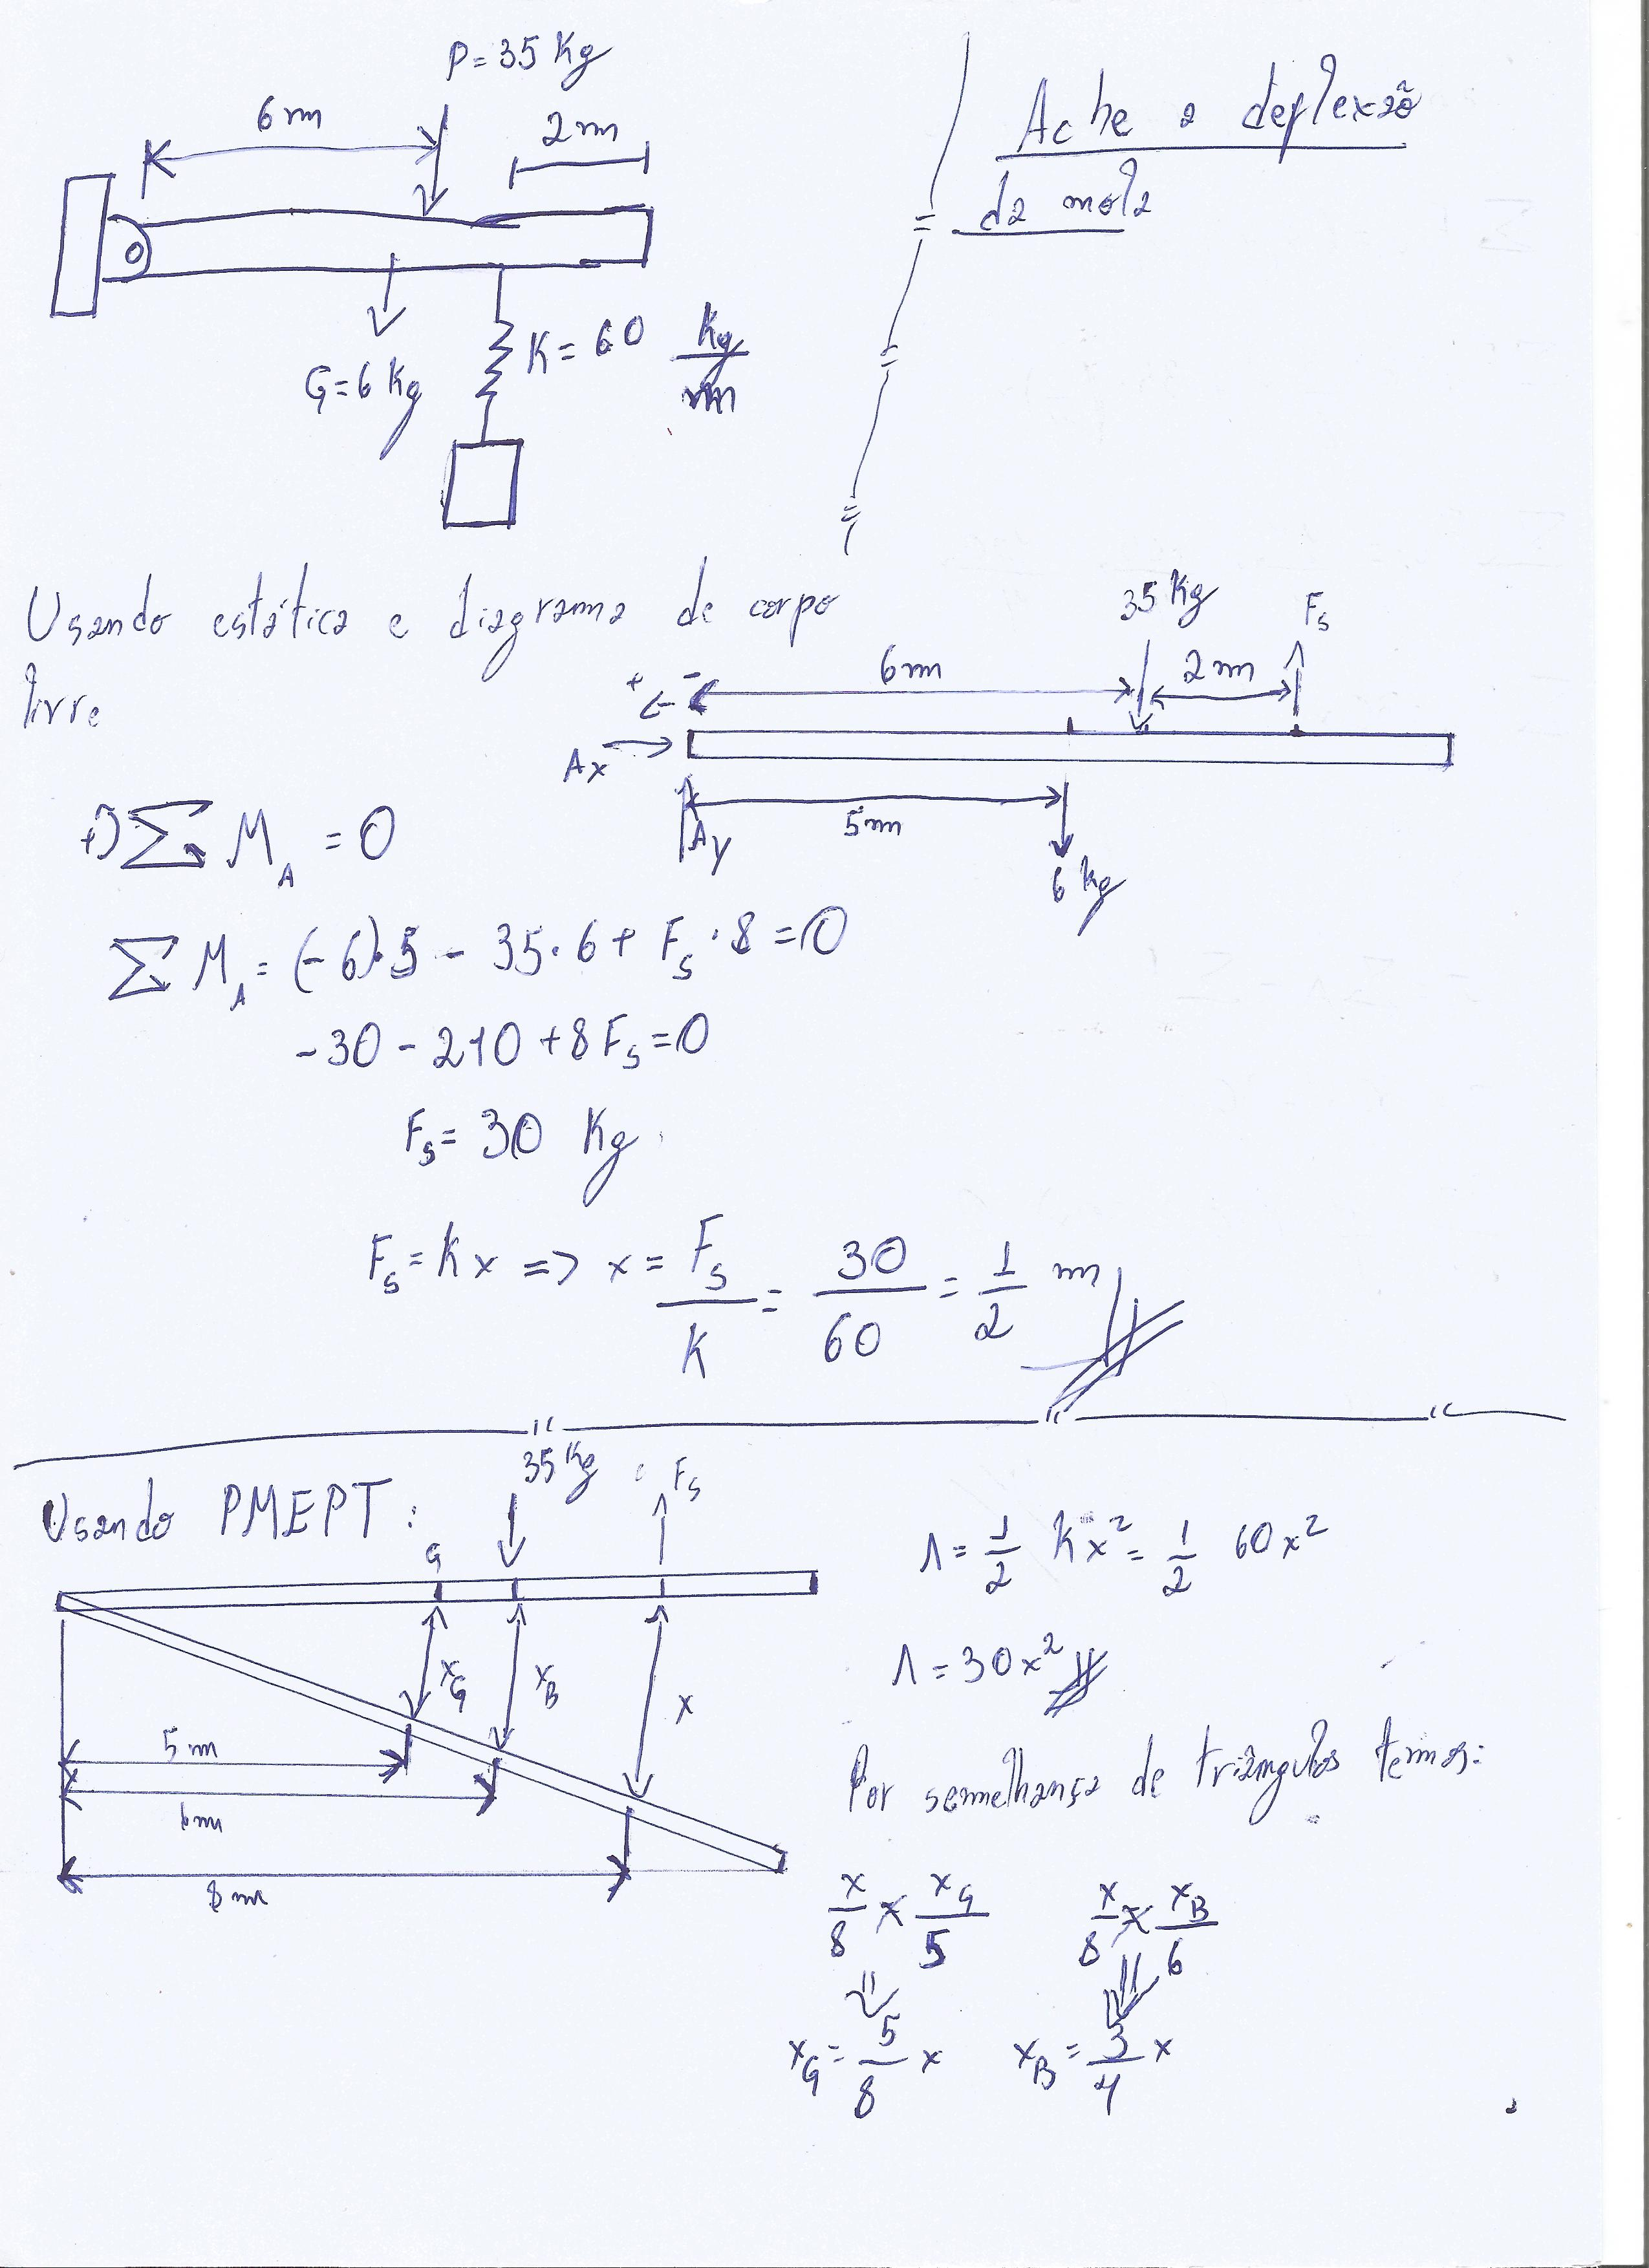
\includegraphics[width=\linewidth]{ResolucaoCasoAnalitico-2.jpg}
\end{figure}%

\begin{figure}[H]
  \centering
  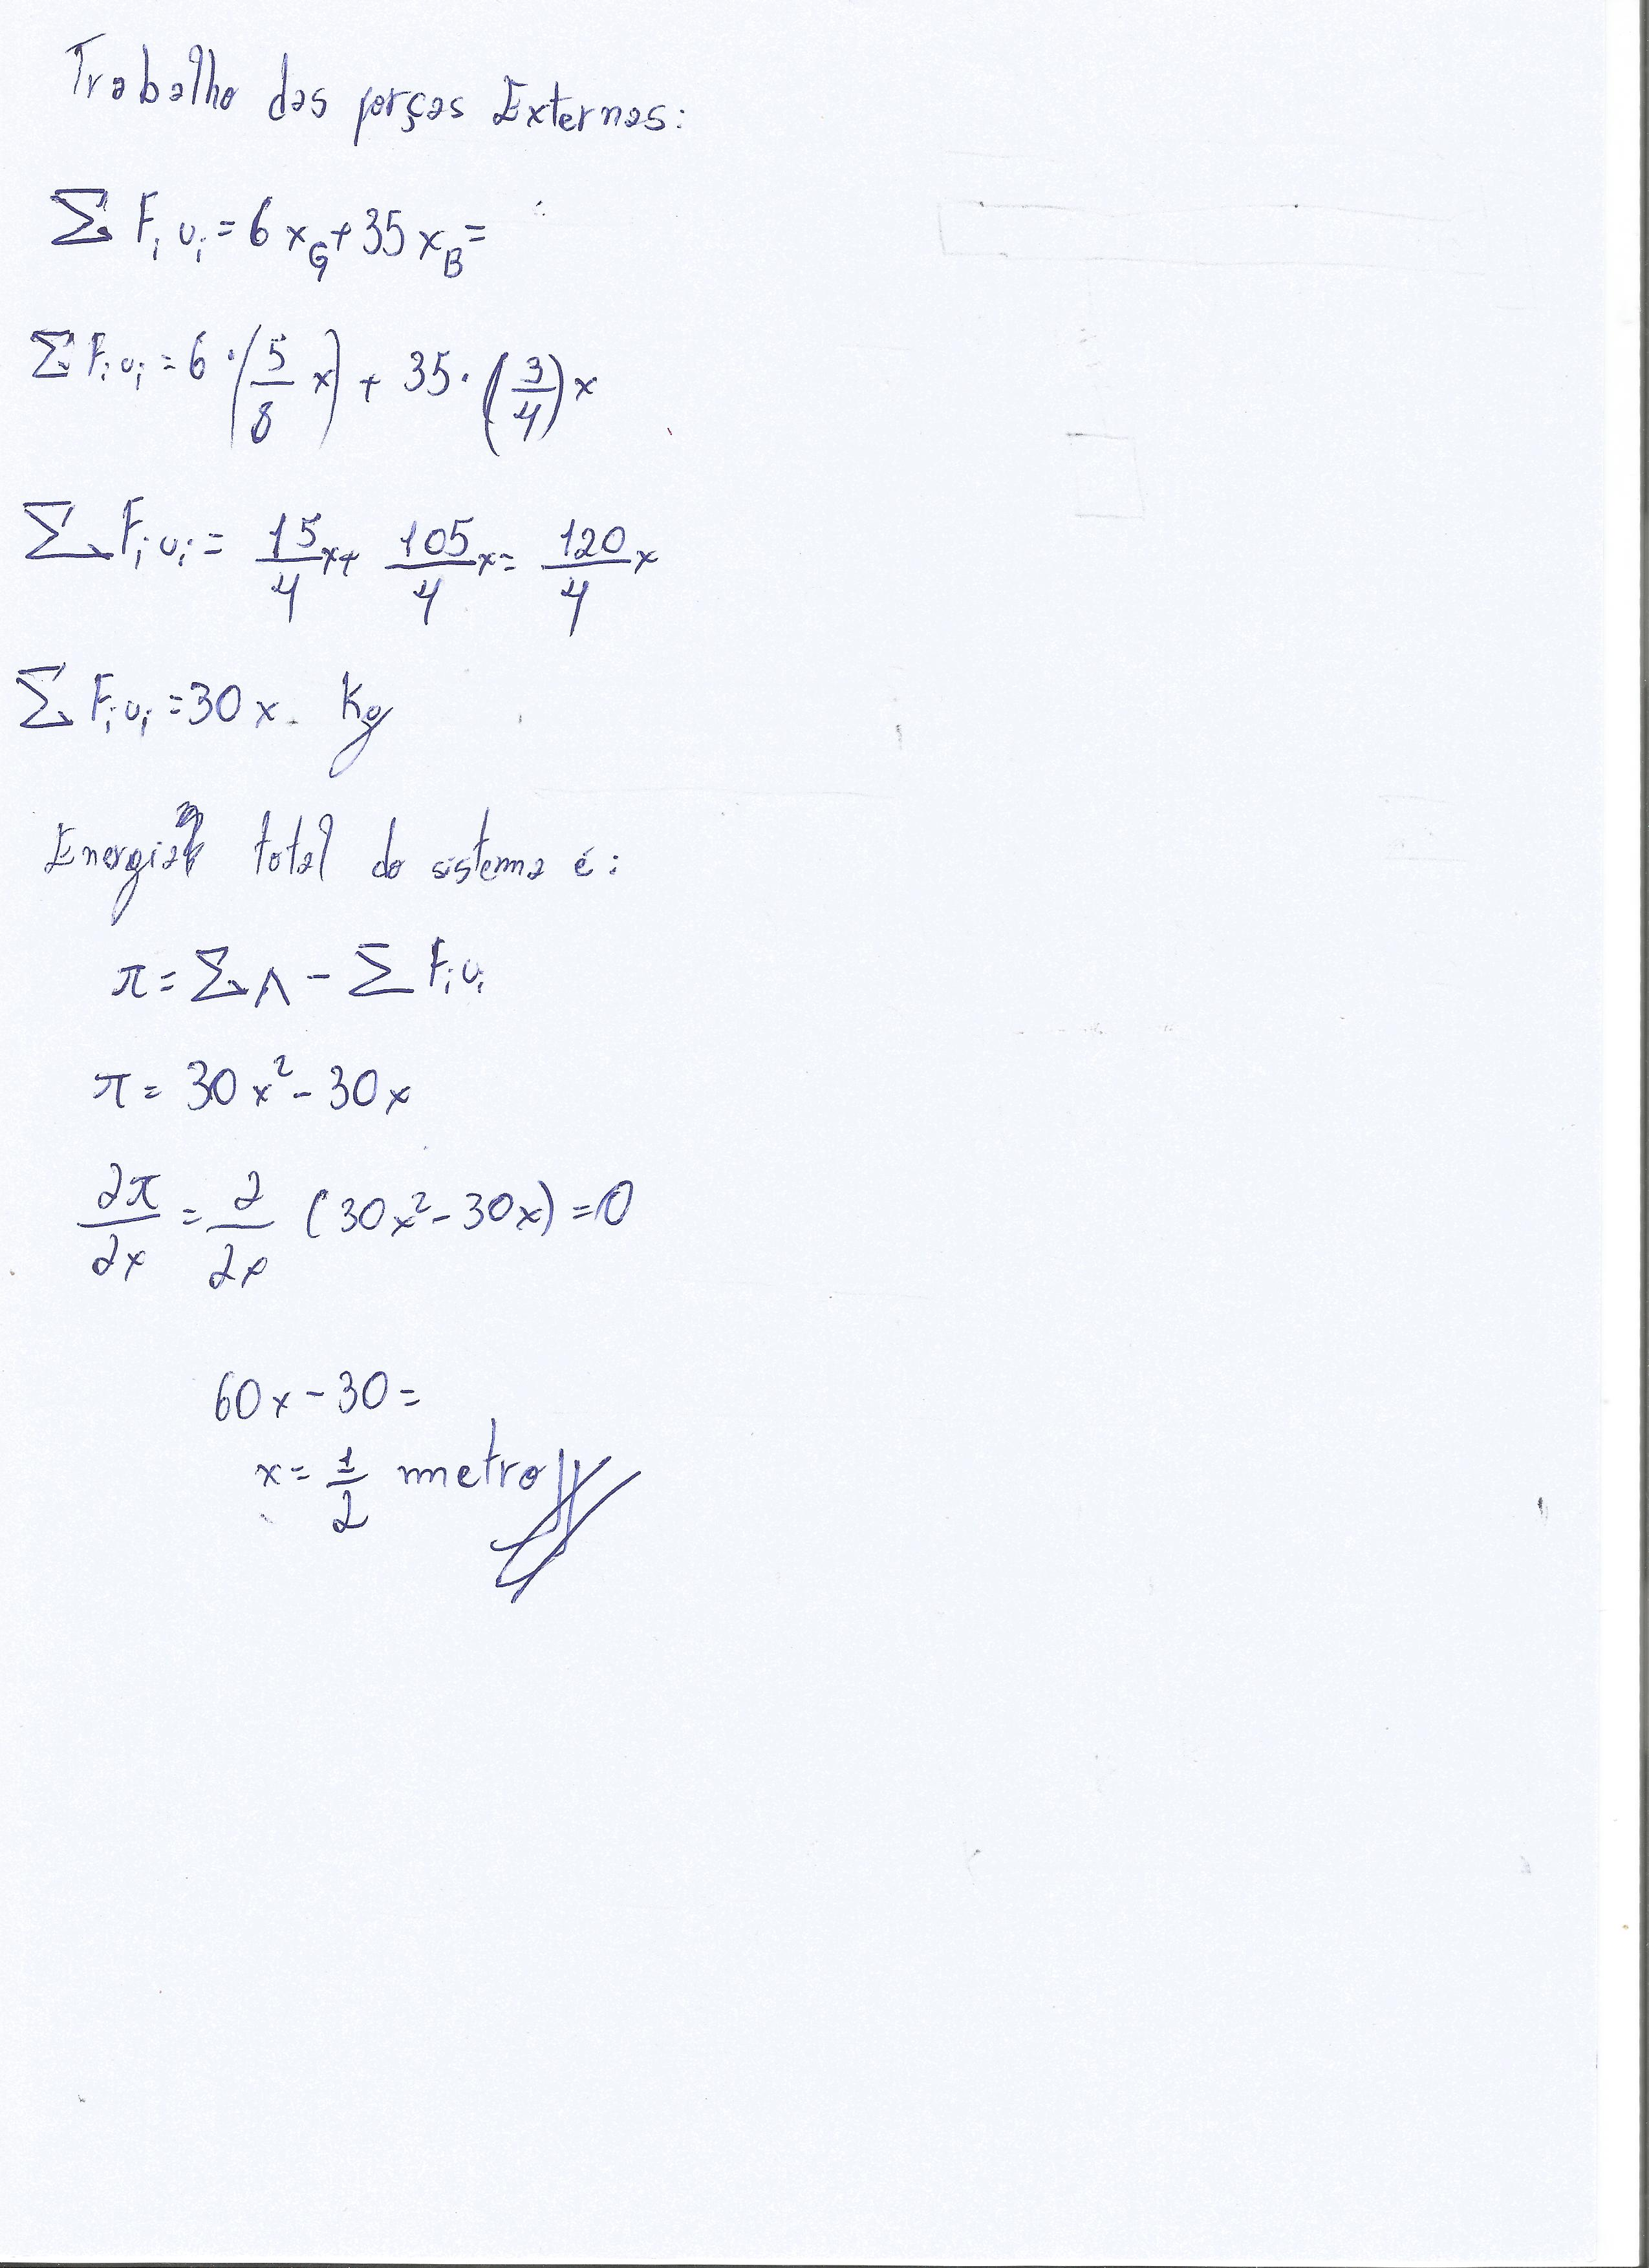
\includegraphics[width=\linewidth]{ResolucaoCasoAnalitico-1.jpg}
\end{figure}%


\subsection{Modelagem da treliça simplesmente engastada}
O modelo busca representar a deformação de uma estrutura engastada em apenas um dos lados (cantilever) utilizando-se de uma abordagem de otimização para este fim. Logo, é necessário escrever uma função objetivo que relacione as variáveis de estado do sistema a energia potencial do sistema. Considera-se que a estrutura é um sistema massa-mola discretizado em forma de malha, com as seguintes características:

\begin{itemize}
\item O sistema possui 2 graus de liberdade;
\item Considera-se que a viga é constituída de $n$ massas (nós), conectadas por $2n-3$
molas (elementos de malha triangulares);
\item Rigidez da estrutura e módulo de elasticidade são definidos em função da
rigidez e comprimento relaxado das molas.
\item As molas podem se deformar infinitamente (i.e: o modelo não representa
rompimento).
\end{itemize}

Logo, a energia potencial total do sistema é dada pela soma da energia potencial elástica e a energia potencial gravitacional de cada/entre cada nó (\cite{liu2013fast}). Abaixo foram listadas as 2 equações fundamentais do modelo.\newline

Energia potencial de uma mola entre dois pontos:
\begin{equation}
\begin{split}
\frac{1}{2} k( (|p_1 - p_2|) - r)^2
\end{split}
\end{equation}

Energia potencial total de uma massa:
\begin{equation}
\begin{split}
E_{pg} = mgh
\end{split}
\end{equation}



Para um sistema com $n$ massas, generaliza-se os índices das fórmulas, e, obtêm-se a seguinte função objetivo:
\begin{equation}
\begin{split}
min \,\,\,\, U & = \sum_{i=1}^{n} mgy_i + \frac{1}{2} \sum_{i,j=1}^{n} k a_{ij} (|p_i - p_j| - l_{ij})^2 \,\, s.t: \\
p_1 & = (0.0, 0.0) \\
p_2 & = (0.0, -0.1) \\
p_i & - 1.0 \leq p_i \leq p_i + 1.0  \,\, , i = 3, ... , n ,\,\ (opcional)
\end{split}
\end{equation}

\begin{itemize}
\item $n$ -- quantidade de nós da malha;
\item $m$ -- massa sobre a estrutura ($kg$);
\item $g$ -- constante gravitacional ($m/s$);
\item $y_i$ -- coordenada y do nó (matriz coluna);
\item $k$ -- constante elástica das molas ($kg/m$);
\item $p_i$ -- i-ésima posição (x,y) do nó (matriz);
\item $a_{ij}$ -- elemento da matriz de adjacência (1 caso exista mola, 0 senão);
\item $l_{ij}$ -- comprimento relaxado da mola (i,j) (0 caso não exista mola entre nós) (matriz);
\end{itemize}
As restrições do problema de otimização representam as condições de contorno do sistema.
\section{Algoritmos utilizados}
\subsection{L-BFGS-B}

O algoritmo L-BFGS-B (\cite{zhu1997algorithm}) é uma modificação do algoritmo BFGS capaz de lidar com limites laterais 
(i.e: $a \leq x \leq b$) diretamente. Além disso, este algoritmo não armazena uma aproximação densa da inversa da 
matriz hessiana, ao invés disso, o algoritmo armazena apenas alguns vetores que representam tal termo implicitamente, 
i.e: o algoritmo armazena as últimas $m$ atualizações de $x$ e $\nabla f(x)$. Estes termos são utilizados quando 
algumas operações exigem o produto vetorial da matriz $H_k$. \newline
O tratamento dos limites laterais é realizado através do método de gradiente que identifica o conjunto com os limites 
das variáveis de entrada que estão ativas, e então o modelo quadrático é aproximadamente minimizado, em relação as 
variáveis livres.

Após isso, o próximo ponto de avaliação é calculado através da busca unidimensional, utilizando um
determinado tamanho de passo $\alpha_{l-bfgs-b}$ (hiperparâmetro).
\subsection{SLSQP}
O SLSQP (Sequential Least Squares Quadratic Programming) (\cite{wendorff2016comparing}) é um algoritmo de programação sequencial de mínimos quadrados. O SLSQP usa o algoritmo BFGS para aproximar a Hessiana e a função de mérito $L$ é usada para uma busca unidimensional. 

As restrições de desigualdade e igualdade são combinadas e expressadas por $\overrightarrow{h_k}$, o vetor de 
multiplicadores de Lagrange é dado por $u_k$. As restrições de desigualdade são igualadas a zero e tratadas de acordo 
(entretanto os multiplicadores de Lagrange associados a estas restrições não devem ser negativos),  restrições de 
desigualdade inativas são ignoradas. 

Existem 3 critérios de parada para o algoritmo SLSQP, são eles:

\begin{eqfloat}[H]
\begin{equation}
\begin{split}
|\nabla f_k^T d_k| + \sum |u_i| |h_i(x_k)| \leq tol
\end{split}
\end{equation}
\caption{Condição de Parada 1}
\label{eqn:cp1}
\end{eqfloat}

\begin{eqfloat}[H]
\begin{equation}
\begin{split}
|f(x)_k - f(x)_{k+1}| \leq tol
\end{split}
\end{equation}
\caption{Condição de Parada 2}
\label{eqn:cp2}
\end{eqfloat}

\begin{eqfloat}[H]
\begin{equation}
\begin{split}
k \geq \text{max it}
\end{split}
\end{equation}
\caption{Condição de Parada 3}
\label{eqn:cp3}
\end{eqfloat}

Como pode ser visto pela equação 9 O tamanho do primeiro passo da busca unidimensional geralmente é 1, este tamanho de passo é reduzido sucessivamente por um determinado fator de contração. Logo, o primeiro termo $| \nabla f_k^T d_k|$ representa  representa o quanto de melhoria a função objetivo obteve ao longo da direção de descida mais íngreme com o maior comprimento de passo.
O segundo termo representa uma combinação ponderada do total de todas as violações. Portanto, este critério
denota que, uma vez que ocorreu uma melhoria significativa da função Lagrangeana $L$ menor que uma tolerância pré-definida, então considera-se que o algoritmo convergiu para um $x*$.\newline

O critério de parada 10 e 11 são amplamente conhecidos, e denotam respectivamente a parada do algoritmo em função da diferença entre dois $x_k$ de iterações consecutivas ser menor que uma tolerância pré-definida, e a parada do algoritmo após um número máximo de iterações.\newline




A função de mérito $L_1$ (equação \ref{eqn:L1}) é utilizada para garantir uma convergência global, o que significa que o $x$ ótimo será encontrado, independentemente do $x$ inicial. A função de mérito pode ser considerada como uma função objetivo para a busca unidimensional, esta é decrementada sucessivamente para a geração de um novo $x_k$ no decorrer do processo. Para problemas irrestritos a função objetivo original pode ser usada como função de mérito, em qualquer outro caso, a função de mérito $L_1$ assume a seguinte forma:

\begin{eqfloat}[H]
\begin{equation}
\begin{split}
L_1 = f(x_k + \alpha d_k) + \sum_{j=1}^{m} \rho_j |h_i (x_k + \alpha d_k)|
\end{split}
\end{equation}
\caption{Função de mérito L1}
\label{eqn:L1}
\end{eqfloat}

O fluxograma abaixo demonstra o funcionamento básico do algoritmo SLSQP:



\begin{figure}[H]
  \centering
  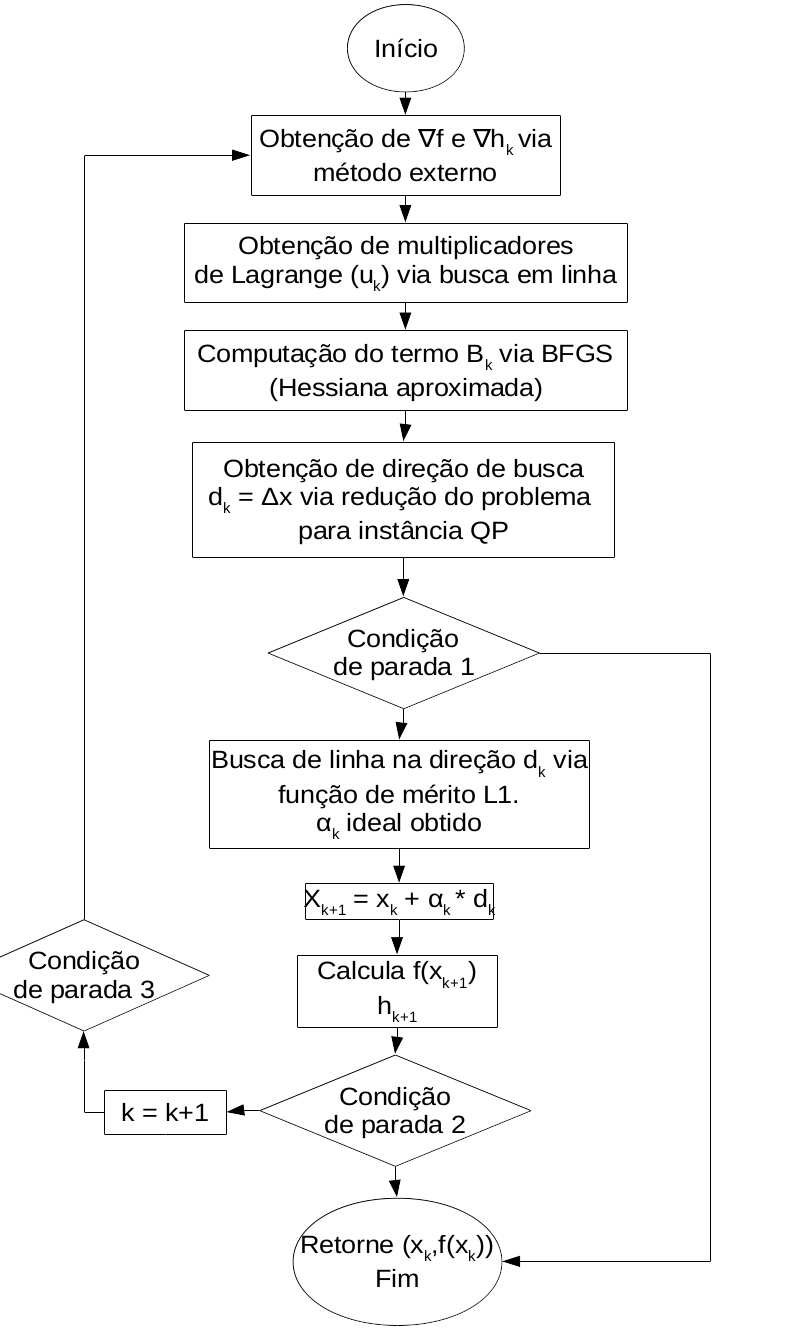
\includegraphics[width=0.7\linewidth]{slsqp.png}
  \caption{Fluxograma do algoritmo SLSQP}
\end{figure}


\subsection{Método de Newton Truncado}
O método de Newton truncado (\cite{schlick1987powerful}) é um algoritmo de otimização que, dado um $x_k$, aproxima um $x*$ resolvendo as equações de Newton (...) usando algum algoritmo iterativo com precondicionamento $M^k$. $M^k$ é escolhido com informação de algum outro algoritmo de otimização (geralmente gradiente conjugado) ou com base em iterações anteriores. Usando a solução obtida para as equações de Newton, uma direção de descida é computada, e uma nova aproximação $x_{k+1}$ de $x*$ é obtida. As equações de Newton são definidas da seguinte forma:

Considerando que a função objetivo é aproximada por uma série de Taylor, temos:
\begin{equation}
\begin{split}
F(x^{(0)} + p) = F(x^{(0)}) + p^T \nabla F(x^{(0)} + \frac{1}{2} p^T \nabla^2 F(x^{(0)}) p + R_3 (x^{(0)}, p)
\end{split}
\end{equation}

onde $R_3(x^{(0)}, p)$ representam os termos de alta ordem da série. Logo, as equações de Newton são dadas pela fórmula abaixo:

\begin{equation}
\begin{split}
Hp = -g
\end{split}
\end{equation}

Onde $H$ é a matriz Hessiana, $g$ é o gradiente de $f$ e $p$  é o ponto de interesse da série.
\subsection{Evolução Diferencial}
O algoritmo de Evolução Diferencial (\cite{storn1997differential}) é um algoritmo de otimização simples e eficiente que foi proposto por Rainer Storn e Kenneth Price em 1995. Mostra-se eficaz para funções objetivo que não são diferenciáveis ou convexas e tem facilidade na busca do ótimo com populações pequenas.
O DE pode ser descrito como uma manipulação de indivíduos que representam as soluções candidatas. No decorrer das gerações, essas soluções candidatas sofrem modificações de mutação e cruzamento, onde são geradas novas soluções candidatas, e logo após é feita a seleção e o ciclo se repete. A figura \ref{fig:EDTeoria} demonstra o funcionamento básico do algoritmo de Evolução Diferencial

\begin{figure}[H]
  \centering
  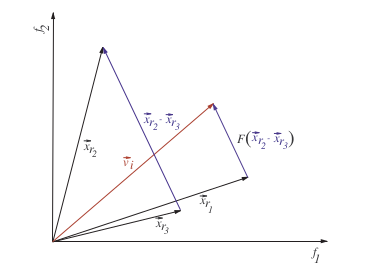
\includegraphics[width=0.5\linewidth]{EDteoria.png}
  \caption{Funcionamento da Evolução Diferencial -- \cite{storn1997differential}}
  \label{fig:EDTeoria}
\end{figure}%


Partindo de três vetores $\overrightarrow{x_{r1}}$ , $\overrightarrow{x_{r2}}$ e $\overrightarrow{x_{r3}}$, são escolhidos
aleatoriamente dois deles (nesse caso $\overrightarrow{x_{r2}}$ e $\overrightarrow{x_{r3}}$), sendo realizada a subtração dos mesmos. O resultado é 
multiplicado por um escalar $F$ , gerando assim um vetor com módulo diferente da subtração original. Esse novo vetor 
é então somado ao vetor $\overrightarrow{x_{r1}}$ , fornecendo assim um novo vetor $\overrightarrow{v_i}$ . Esse vetor $\overrightarrow{v_i}$ indicará uma nova posição 
no espaço, ou um novo indivíduo (muito semelhante a um algoritmo genético, mas com cromossomos compostos por valores 
reais).
\section{Resultados}
Para a documentação neste relatório, foi elaborado o experimento abaixo:\newline

Parâmetros do experimento 1:
\begin{itemize}
\item massa  -- $m = 0.1$;
\item número de nós  -- $n = 20$;
\item distância inicial entre nós -- $e = 0.1$;
\item comprimento das molas em situações sem deformação -- $l = 0.1$;
\item constante de rigidez da mola $k = 10000$
\end{itemize}
As próximas seções documentam os resultados obtidos.
\subsection{Métodos Clássicos}

Configuração inicial da treliça:

\begin{figure}[H]
  \centering
  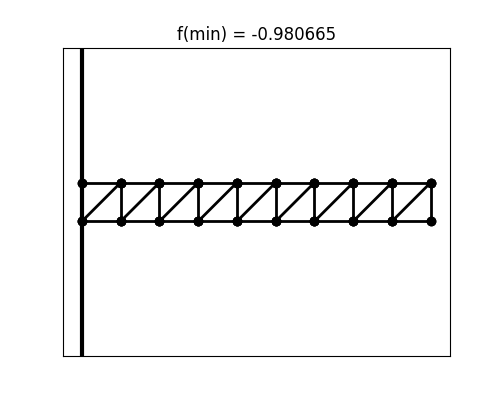
\includegraphics[width=0.5\linewidth]{experimento1_configuracao_inicial.png}
  \caption{Representação gráfica da configuração inicial da treliça}
\end{figure}



\begin{longtable}[c]{|l|l|l|l|l|}
\hline
\multicolumn{1}{|c|}{\cellcolor[HTML]{FFFFFF}{\color[HTML]{000000} Métodos x Métricas}} & \multicolumn{1}{c|}{Qtde de variáveis} & \multicolumn{1}{c|}{Qtde de Iterações} & \multicolumn{1}{c|}{\begin{tabular}[c]{@{}c@{}}Avaliações da função\\ objetivo\end{tabular}} & \multicolumn{1}{c|}{Min F(x)} \\ \hline
\endfirsthead
%
\multicolumn{5}{c}%
{{\bfseries Continuação da tabela \thetable\ }} \\
\hline
\multicolumn{1}{|c|}{\cellcolor[HTML]{FFFFFF}{\color[HTML]{000000} Métodos x Métricas}} & \multicolumn{1}{c|}{Qtde de variáveis} & \multicolumn{1}{c|}{Qtde de Iterações} & \multicolumn{1}{c|}{\begin{tabular}[c]{@{}c@{}}Avaliações da função\\ objetivo\end{tabular}} & \multicolumn{1}{c|}{Min F(x)} \\ \hline
\endhead
%
L-BFGS-B                                                                                    & 40 (20 nós)                            & 133                                    & 138                                                                                          & -2.52938265048                \\ \hline
SLSQP                                                                                     & 40 (20 nós)                            & 58                                     & 2557                                                                                         & -2.529382692846               \\ \hline
Newton Truncado                                                                         & 40 (20 nós)                            & 830                                    & 62                                                                                           & -2.51249006635                \\ \hline
\caption{Resultados obtidos no experimento 1}
\label{tab:Experimento1-Classico}\\
\end{longtable}
\begin{figure}[H]
\centering
\begin{subfigure}{0.3\textwidth}
  \centering
  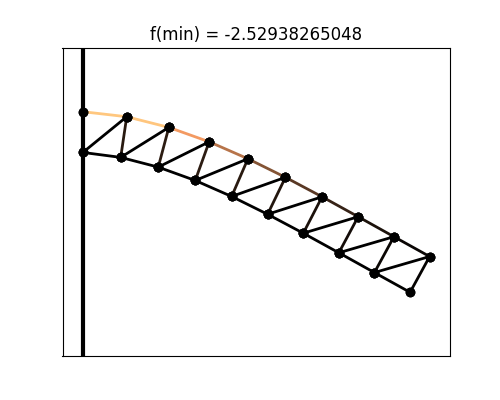
\includegraphics[width=\linewidth]{experimento1_LBFGSB.png}
  %\caption{A subfigure}
\end{subfigure}%
\begin{subfigure}{0.3\textwidth}
  \centering
  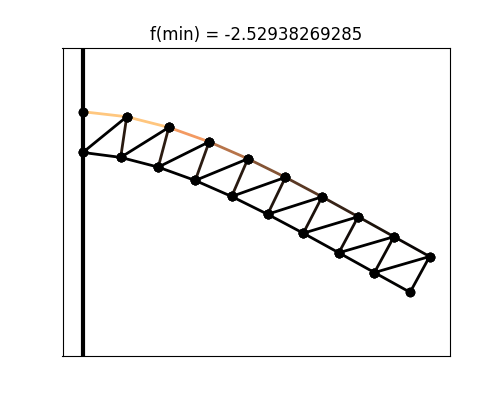
\includegraphics[width=\linewidth]{experimento1_SQP.png}
  %\caption{A subfigure}
\end{subfigure}
\begin{subfigure}{0.3\textwidth}
  \centering
  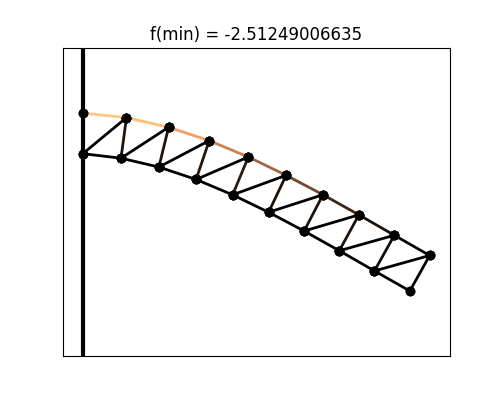
\includegraphics[width=\linewidth]{experimento1_TNC.png}
  %\caption{A subfigure}
\end{subfigure}
\caption{Configuração Final da treliça computada pelo Algoritmo L-BFGS-B, SLSQP e Newton Truncado respectivamente}
\label{fig:Q6BFGS}
\end{figure}


% Please add the following required packages to your document preamble:
% \usepackage{longtable}
% Note: It may be necessary to compile the document several times to get a multi-page table to line up properly
\begin{longtable}[c]{|l|l|}
\hline
x                        & y                         \\ \hline
\endfirsthead
%
\multicolumn{2}{c}%
{{\bfseries Continuação da tabela \thetable\ }} \\
\hline
x                        & y                         \\ \hline
\endhead
%
0.000000000000000000e+00 & 0.000000000000000000e+00  \\ \hline
0.000000000000000000e+00 & -1.000000000000000056e-01 \\ \hline
1.076604963454961816e-01 & -1.234808813968935916e-02 \\ \hline
9.285609344426656864e-02 & -1.121326312494193983e-01 \\ \hline
2.110453836830193108e-01 & -3.846447531552332072e-02 \\ \hline
1.850558031116051882e-01 & -1.360255187418834555e-01 \\ \hline
3.100610838664475399e-01 & -7.385988911778323951e-02 \\ \hline
2.758761475637592775e-01 & -1.688408715429658424e-01 \\ \hline
4.052258921423890214e-01 & -1.154953481559722744e-01 \\ \hline
3.652746997896266223e-01 & -2.081062035747603123e-01 \\ \hline
4.973522619098407760e-01 & -1.610865755944085043e-01 \\ \hline
4.535493330435532711e-01 & -2.518005457540001268e-01 \\ \hline
5.873054061940690129e-01 & -2.089383588685599091e-01 \\ \hline
5.411242112703530394e-01 & -2.982980063307638652e-01 \\ \hline
6.758761883112499591e-01 & -2.578169836431673523e-01 \\ \hline
6.284127007501388862e-01 & -3.463189503723093643e-01 \\ \hline
7.637177846436586925e-01 & -3.068631367068182514e-01 \\ \hline
7.157347676073907428e-01 & -3.948925412627222187e-01 \\ \hline
8.513196221584131695e-01 & -3.555422158899081975e-01 \\ \hline
8.032695093465200831e-01 & -4.433394937483930431e-01 \\ \hline
\caption{Posições finais dos nós computados pelo L-BFGS-B}
\label{tab:experimento1-lbfgsb}\\
\end{longtable}

% Please add the following required packages to your document preamble:
% \usepackage{longtable}
% Note: It may be necessary to compile the document several times to get a multi-page table to line up properly
\begin{longtable}[c]{|l|l|}
x                        & y                          \\ \hline
\endfirsthead
%
\multicolumn{2}{c}%
{{\bfseries Continuação da tabela \thetable\ }} \\
x                        & y                          \\ \hline
\endhead
%
0.000000000000000000e+00 & 0.000000000000000000e+00 \\ \hline
0.000000000000000000e+00 & -1.000000000000000056e-01 \\ \hline
1.076581016588509659e-01 & -1.234252877187444822e-02 \\ \hline
9.285697905639224425e-02 & -1.121273723211763246e-01 \\ \hline
2.110435483900849618e-01 & -3.845261169162977194e-02 \\ \hline
1.850589607610042264e-01 & -1.360139709305897282e-01 \\ \hline
3.100614950867626729e-01 & -7.383759639200435099e-02 \\ \hline
2.758808407504163562e-01 & -1.688194012225558427e-01 \\ \hline
4.052274160172885109e-01 & -1.154721206354224761e-01 \\ \hline
3.652794197173069302e-01 & -2.080853121149189855e-01 \\ \hline
4.973554329820704112e-01 & -1.610579591497134644e-01 \\ \hline
4.535571696553672427e-01 & -2.517734303334946966e-01 \\ \hline
5.873107838861030272e-01 & -2.089042278612215919e-01 \\ \hline
5.411329922867171849e-01 & -2.982663049064730454e-01 \\ \hline
6.758827785101579888e-01 & -2.577831678481600219e-01 \\ \hline
6.284233764303035485e-01 & -3.462874535685726007e-01 \\ \hline
7.637250577912088056e-01 & -3.068229353638805001e-01 \\ \hline
7.157473943252998794e-01 & -3.948549020339718885e-01 \\ \hline
8.513293735802619500e-01 & -3.554980033699064457e-01 \\ \hline
8.032843643335488837e-01 & -4.432975511277799652e-01 \\ \hline
\caption{Posições finais dos nós computados pelo SLSQP}
\label{tab:experimento1-sqp}\\
\end{longtable}

% Please add the following required packages to your document preamble:
% \usepackage{longtable}
% Note: It may be necessary to compile the document several times to get a multi-page table to line up properly
\begin{longtable}[c]{|l|l|}
\hline
x                        & y                         \\ \hline
\endfirsthead
%
\multicolumn{2}{c}%
{{\bfseries Continuação da tabela \thetable\ }} \\
\hline
x                        & y                         \\ \hline
\endhead
%
0.000000000000000000e+00 & 0.000000000000000000e+00  \\ \hline
0.000000000000000000e+00 & -1.000000000000000056e-01 \\ \hline
1.073453320603787731e-01 & -1.131906141904176315e-02 \\ \hline
9.390695378617000544e-02 & -1.111144547211459221e-01 \\ \hline
2.109855703932395077e-01 & -3.505453679425795527e-02 \\ \hline
1.871162548763355415e-01 & -1.329081016022125861e-01 \\ \hline
3.109290112846055387e-01 & -6.796005448866306031e-02 \\ \hline
2.786578919106891261e-01 & -1.634131799516077566e-01 \\ \hline
4.072288059110498737e-01 & -1.080791236868817312e-01 \\ \hline
3.685794437575616311e-01 & -2.012766910145951105e-01 \\ \hline
5.002811533915770825e-01 & -1.532024195396144706e-01 \\ \hline
4.570264280056981487e-01 & -2.440769482580765759e-01 \\ \hline
5.908554038684504794e-01 & -2.009954397605685228e-01 \\ \hline
5.443707874541260372e-01 & -2.902751946570642505e-01 \\ \hline
6.792081549818771435e-01 & -2.504898803189012924e-01 \\ \hline
6.309492576946710285e-01 & -3.387666102692873382e-01 \\ \hline
7.663160328145873779e-01 & -3.007088386085366438e-01 \\ \hline
7.175186124147107103e-01 & -3.884533589826867916e-01 \\ \hline
8.533262796408570550e-01 & -3.504586983865930483e-01 \\ \hline
8.045345136075724435e-01 & -4.377923103295616736e-01 \\ \hline
\caption{Posições finais dos nós computados pelo Método de Newton Truncado}
\label{tab:experimento1-tnc}\\
\end{longtable}

\subsection{Métodos Evolutivos}

\begin{figure}[H]
\centering
\begin{subfigure}{0.5\textwidth}
  \centering
  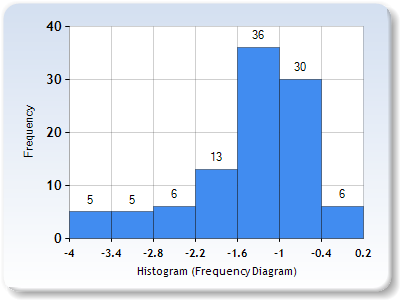
\includegraphics[width=\linewidth]{experimento1.png}
  %\caption{A subfigure}
\end{subfigure}%
\begin{subfigure}{0.5\textwidth}
  \centering
  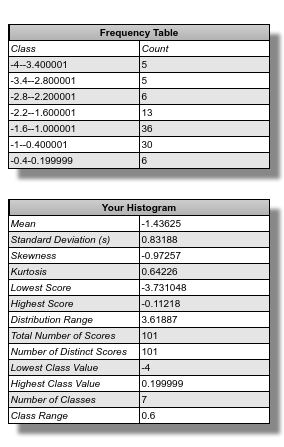
\includegraphics[width=\linewidth]{_experimento1.png}
  %\caption{A subfigure}
\end{subfigure}
\caption{Histograma e análise estatística da resposta do algoritmo de Evolução Diferencial para uma população de 40 candidatos}
\label{fig:evolutivo1}
\end{figure}


\begin{figure}[H]
\centering
\begin{subfigure}{0.5\textwidth}
  \centering
  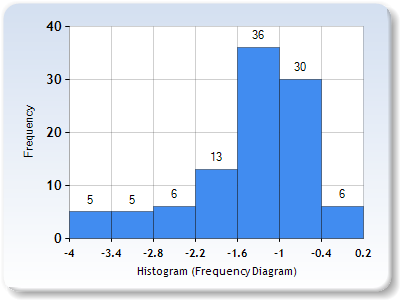
\includegraphics[width=\linewidth]{experimento1.png}
  %\caption{A subfigure}
\end{subfigure}%
\begin{subfigure}{0.5\textwidth}
  \centering
  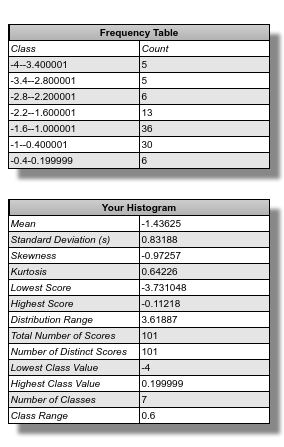
\includegraphics[width=\linewidth]{_experimento1.png}
  %\caption{A subfigure}
\end{subfigure}
\caption{Histograma e análise estatística da resposta do algoritmo de Evolução Diferencial para uma população de 100 candidatos}
\label{fig:evolutivo2}
\end{figure}

\subsection{Discussões}
Dentre os algoritmos clássicos, nota-se que o algoritmo L-BFGS-B obteve uma performance superior ao Método de Newton Truncado, visto que este obteve o melhor trade-off entre número de iterações e número de avaliações da função objetivo. Ao passo que o L-BFGS-B era superado pelo Newton Truncado em número de avaliações da função objetivo (45\% a mais), este o superava em iterações (83\% a menos). Similarmente o L-BFGS-B superou o SLSQP, visto que o L-BFGS-B levou 133 iterações para convergir ao ótimo, enquanto o SLSQP necessitou de apenas 58. Em contra-partida, o SLSQP necessitou de 2557 avaliações da função objetivo, enquanto que o L-BFGS-B necessitou de apenas 138 avaliações da função objetivo.\newline
A superioridade do L-BFGS-B é mantida para configurações iniciais mais complexas, tornando-o o método ideal para a resolução deste tipo de problema.\newline
No que tange a métodos evolutivos, a Evolução Diferencial foi escolhida devido ao fato deste algoritmo necessitar de pequenas populações (quando comparados a outros métodos evolutivos) para atingir a convergência. Em testes preliminares, outros algoritmos evolutivos necessitaram de muito tempo para gerar uma população de indíviduo (geralmente um vetor com 20 posições), e realizar operações de mutação e similares. Infelizmente o algoritmo de Evolução Diferencial não foi capaz de resolver o problema original, sendo necessário adicionar mais restrições laterais ao mesmo, da forma:

\begin{equation}
\begin{split}
-i \mod 2 \leq p_{i+2} \leq (i \mod 2) -1 ,\ i = 0, 1, ..., n-2
\end{split}
\end{equation}

Onde tais limites são relativos as posições iniciais de cada nó. Após isto, foram realizados dois testes com tamanhos de população de 40 e 100 candidatos. Em ambos os casos foi utilizada amostragem por hipercubo latino, a fim de que a população de vetores iniciais cobri-se o espaço de busca da melhor maneira possível. As taxas de recombinação foram respectivamente 0.7 e 0.5\newline
Nota-se que o aumento da população e a diminuição da taxa de recombinação levou o algoritmo de Evolução Diferencial a convergir para um resultado correto com mais frequência, mesmo assim ambos os testes as respostas apresentaram uma dispersão substancial das respostas dadas pelo algoritmo evolutivo.
\section{Conclusão}
Concluí-se que o modelo desenvolvido é capaz de associar os estados das variáveis do sistema (campos de deslocamentos) a energiqa potencial total do sistema, possibilitando que o problema de computar a configuração final da estrutura seja feito na forma de problema de otimização. Nota-se que o algoritmo L-BFGS-B mostrou-se mais adequado para a resolução deste problema, visto que este foi capaz de realizar superar o algoritmo SQP no número de avaliações da função objetivo (sendo ligeiramente superado no número de iterações) assim como superar o método de Newton Truncado na quantidade de iterações necessárias para atingir a convergência (sendo ligeiramente superado na quantidade de avaliações da função objetivo). Todos os algoritmos clássicos foram capazes de computar a configuração final da estrutura sob diferentes configurações iniciais com uma margem de erro aceitável. \newline

A Evolução Diferencial foi escolhida principalmente pelo fato de ser capaz de convergir ao $x$ ótimo com populações relativamente pequenas (em comparação a outros métodos evolutivos), este fato foi claramente percebido nos testes, visto que cada solução candidata era um vetor de $40$ variáveis, o que tornava lento o processo de geração de uma nova população. Dentre os algoritmos evolutivos previamente testados, apenas o algoritmo de Evolução Diferencial foi  capaz de realizar a convergência para uma solução (não necessariamente correta) em tempo hábil para o projeto.\newline

Mesmo assim, o algoritmo de Evolução Diferencial teve um resultado insatisfatório neste estudo, devido a necessidade de inserir restrições laterais adicionais a fim de assegurar uma convergência para um resultado correto. Como observado nos histogramas da seção de resultados, os resultados para o algoritmo de Evolução Diferencial foram substancialmente dispersos, até mesmo com o acréscimo do tamanho da população e diminuição da taxa de recombinação/crossover. Além disso, seu custo computacional é alto, devido a grande quantidade de avaliações da função objetivo e geração de candidatos. Conjectura-se que uma mudança na estratégia de mutação do algoritmo (foi utilizada a \textit{best1bin}) possa apresentar melhores resultados.
\bibliographystyle{apalike}
\bibliography{sample}
\end{document}